%%%%%%%%%%%%%%%%%%%%%%%%%%%%%%%%%%%%%%%%%%%%%%%%%%%
%
%  New template code for TAMU Theses and Dissertations starting Fall 2016.
%
%  Author: Sean Zachary Roberson
%	 Version 3.16.09
%  Last updated 9/12/2016
%
%%%%%%%%%%%%%%%%%%%%%%%%%%%%%%%%%%%%%%%%%%%%%%%%%%%
%%%%%%%%%%%%%%%%%%%%%%%%%%%%%%%%%%%%%%%%%%%%%%%%%%%%%%%%%%%%%%%%%%%%%%
%%                           SECTION III
%%%%%%%%%%%%%%%%%%%%%%%%%%%%%%%%%%%%%%%%%%%%%%%%%%%%%%%%%%%%%%%%%%%%%



\chapter{RESULTS}

The results of this research are split into the testing of features and learning algorithms, as detailed in the preceding testing methodology.

\section{Feature Evaluation}
As stated previously, plots of the various distances metrics for features are plotted, along with the corresponding labels, to evaluate whether a feature is sufficient.
Shown below are the plots for pixel distribution, BRIEF descriptors, and blob detection.

\subsection{Pixel Distribution}
Shown is the plot for the Bhattacharyya distances between consecutive image pairs for the feature testing subset:

\begin{figure}[h]
\centering
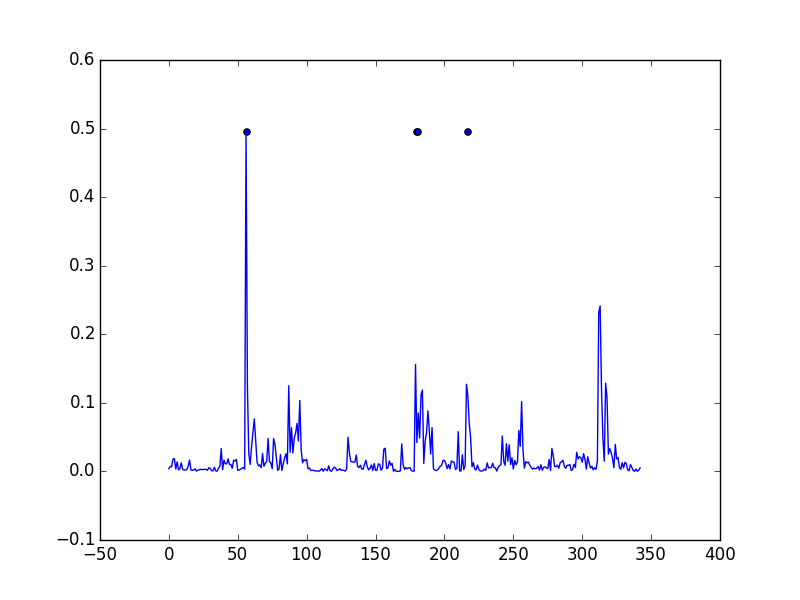
\includegraphics[scale=.50]{figures/611bhattest}
\caption{A general ANN}
\label{fig:tamu-fig3}
\end{figure}

Spikes in the BD can be seen around the locations of the anomalous images, along with some spikes in other areas.

\subsection{BRIEF Descriptors}

First, the plot for the number of BRIEF matches is shown:

\begin{figure}[h]
\centering
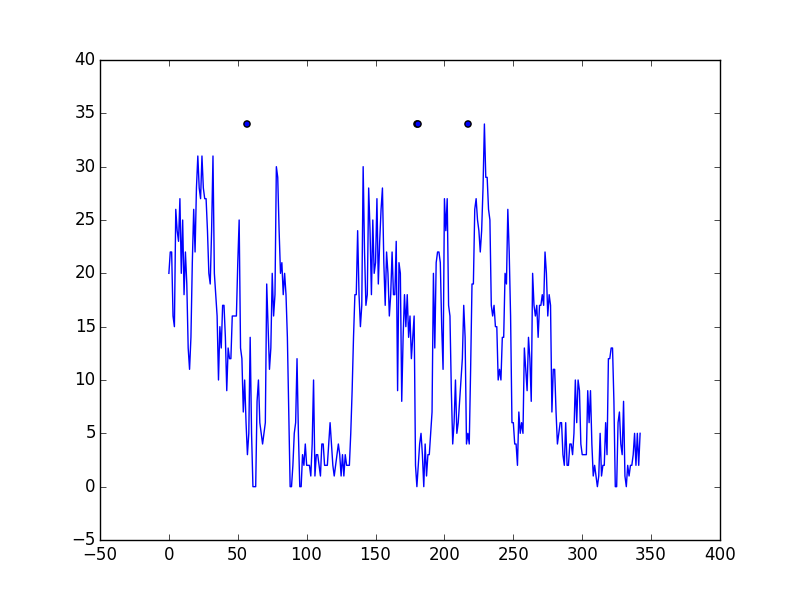
\includegraphics[scale=.50]{figures/611nummatchestest}
\caption{A general ANN}
\label{fig:tamu-fig3}
\end{figure}

Next, the plot for the ratio of keypoints matched is shown:

\begin{figure}[h]
\centering
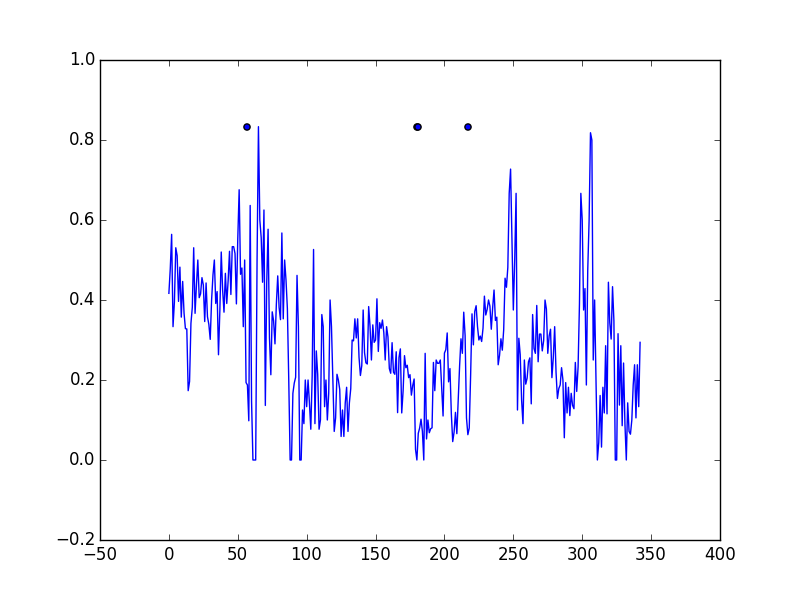
\includegraphics[scale=.50]{figures/611matchratiostest}
\caption{A general ANN}
\label{fig:tamu-fig3}
\end{figure}

Contrary to the other metrics which are true distances, a dip can be seen in the number of matches and the percentage of keypoints matched can be seen around the anomalous images.

\subsection{Blob Detection}

First, the plot for the difference in number of blobs between consecutive images is shown:

\begin{figure}[h]
\centering
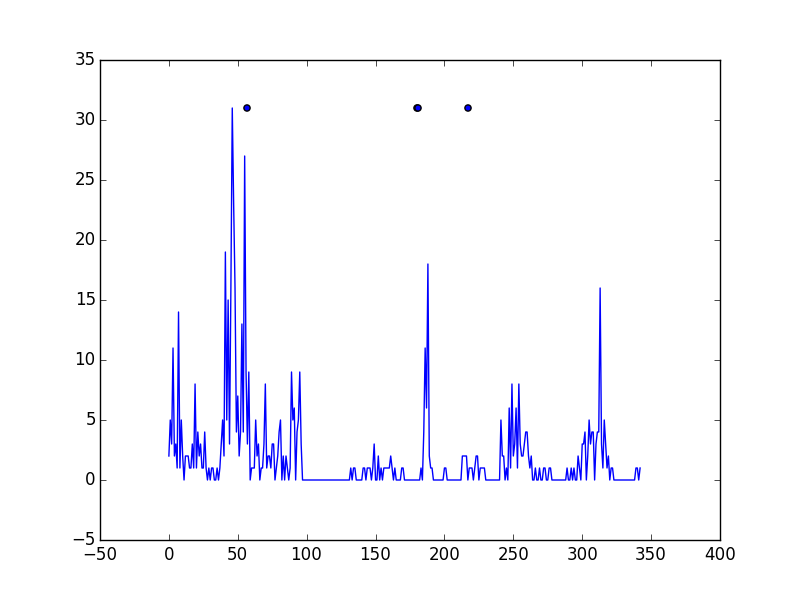
\includegraphics[scale=.50]{figures/blobdiffstest}
\caption{A general ANN}
\label{fig:tamu-fig3}
\end{figure}

Next, the plot for the difference in total blob area between consecutive images is shown:

\begin{figure}[h]
\centering
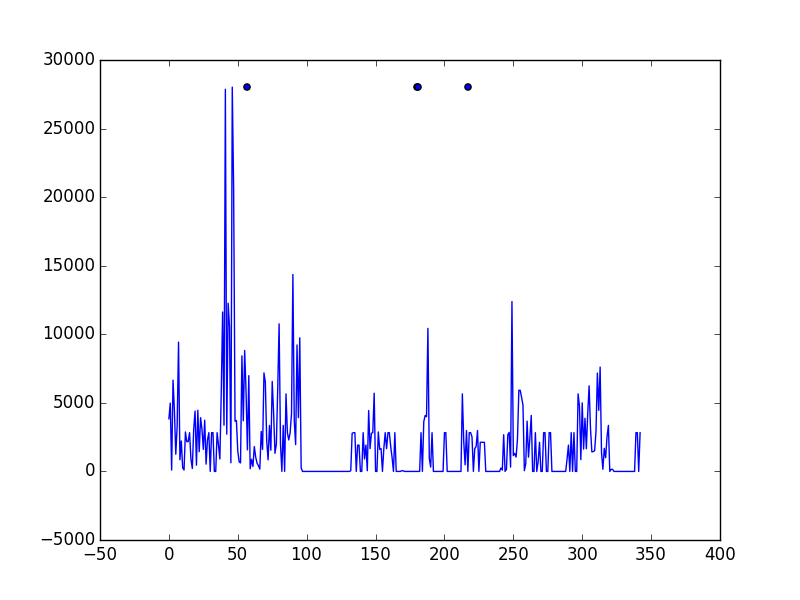
\includegraphics[scale=.50]{figures/blobareadiffstest}
\caption{A general ANN}
\label{fig:tamu-fig3}
\end{figure}

Similarly to the distribution distance plots, spikes can be seen around the anomalous images, as well as in other places.

\section{Learning Algorithm Evaluation}

To evaluate the learning algorithms, these distance metrics were concatenated into feature vectors, and fed along with the corresponding label vector to train each algorithm.
As stated in the testing methodology, the models were then tuned to increase performance, and the final averaged values for detection rate, false alarm rate, and overall accuracy are reported in the table below:

\begin{table}[h!]
	\centering
	\begin{tabular}{|l|l|l|l|}
		\hline
		Algorithm & Detection Rate & False Alarm Rate & Overall Accuracy  \\ \hline
		Logistic Regression & 0.956 & 0.077 & 0.933  \\ \hline
		Decision Trees & 0.119 & 0.033 & 0.899  \\ \hline
		Neural Network & 0.75 & 0.038 & 0.959  \\ \hline
		SVM & 0.924 & 0.258  & 0.743 \\ \hline
	\end{tabular}
	\caption{Performance of learning algorithms in anomalous image detection}
\end{table}


The logistic regression model performed the best out of the four algorithms with a 95.6\% detection rate and a 7.7\% false positive rate.
The decision tree predictably performed poorly, as it is a simple model incapable of considering the interaction between features.
The SVM and neural network had decent performance, with the neural network missing 25\% of anomalous image pairs, and the SVM having a fairly high false alarm rate of 25.8\%.

% \section{Yet Another Table}

% Another table is placed here to show the effect of having tables in multiple sections. The list of tables should still double space between table titles, while single spacing long table titles.

% %Fix table labeling.
% \begin{table}[h!]
% 	\centering
% 	\begin{tabular}{|l|l|}
% 		\hline
% 		Dates & Attendance  \\ \hline
% 		August 8-10, 2008 & 3,523  \\ \hline
% 		August 14-16, 2009 & 4,003 \\ \hline
% 		July 9-11, 2010 & 5,049 \\ \hline
% 		August 5-7, 2011 & 6,891  \\ \hline
% 		August 10-12, 2012 & 9,464  \\ \hline
% 		August 16-18, 2013 & 11,077  \\ \hline
% 		July 18-20, 2014 & 14,686 \\ \hline
% 		July 31-August 2, 2015 & 18,411  \\ \hline
% 	\end{tabular}
% 	\caption{San Japan attendance. Data is taken from \cite{ANCONS}. I intentionally make the title of this table long so the single space effect is seen in the list of tables.}
% \end{table}

% You may be wondering why San Japan was chosen. There are a few reasons as to why I did this:

% \begin{enumerate}
% \item It is one of the fastest-growing anime conventions in Texas.
% \item Filler.
% \item I wanted a good variety of table examples.
% \item Because conventions are cool.
% \end{enumerate}


